In order to understand the motivations for, as well as the limitations, and behaviour of the experiment we need to know about a few key concepts in fluid dynamics.

\subsection{Reynolds Number}
The Reynolds number ($\operatorname{Re}$) is a dimensionless number describing the ratio of inertial forces to viscous forces in a flow. Roughly speaking one can think of viscous forces as acting to keep adjacent fluid elements moving in the same direction whereas inertial forces act to prevent any change in the motion of a fluid element. For a particle in flow it defined as \cite{introfluid}

\begin{equation}\label{eq:reynolds}
\operatorname{Re_p} = \frac{U L \rho}{\mu}
\end{equation}
where $U$ is the characteristic velocity of the flow, $L$ is the characteristic length, $\rho$ is the density of the fluid and $\mu$ is its dynamic viscosity. This is used to estimate the 'regime' of the flow, of which there are two primary types. 
\begin{enumerate}
\item The laminar regime, where viscous forces dominate over inertial forces
\item The turbulent regime where inertial forces dominate.
\end{enumerate}

A simple visual characterization of the flow types can be seen in figure \ref{fig:laminar_flow}. 

 Flow with $\operatorname{Re}\ll 1$ is referred to as \emph{Stokes flow}. In this regime we can ignore inertial forces completely. This has has the implication that not only is the flow guaranteed to be laminar, but it is time reversible.  If there are particles in the flow they will also revert perfectly as long as they too have a Reynolds number that is much smaller than 1~\cite{introfluid3}. 

\begin{figure}[H]
\centering
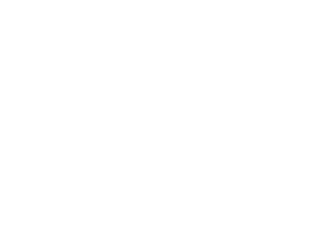
\includegraphics[width=0.6\textwidth]{figures/theory/laminarFlow.pdf}
\caption{This shows the principal difference between laminar and turbulent flow.}
\label{fig:laminar_flow}
\end{figure}


\subsection{Stokes drag and Stokes' law}
The drag force $F_D$ exerted by a fluid on a spherical particle for $\operatorname{Re} \ll 1$ is found using  Stokes's law \cite{introfluid2}

\begin{equation}\label{eq:stokes_law}
F_D = 6\pi \mu R v,
\end{equation}

\noindent where $v$ is the velocity of the sphere relative to the fluid, $\mu$ is the and $R$ is the radius of the sphere. This can be used to find the terminal velocity of a sphere sinking in a liquid by equating the gravitational force $F_G$ acting on the sphere with the drag force from eq \ref{eq:stokes_law}. $F_G$ is calculated as

\begin{equation}
F_G = \Delta \rho g\cdot \frac{4\pi R^3}{3},
\end{equation}

\noindent where $\Delta \rho$ is the difference in density between the fluid and the sphere and $g$ is the specific gravity. We find that the terminal velocity of a sinking (or floating) sphere is

\begin{equation}\label{eq:fallingSphere}
v_s = \frac{2}{9} \frac{\Delta \rho}{\mu} g R^2.
\end{equation}
